\begin{enunciado}{7}
    Plot the bounds for $m_{\hipotset}(N)$ given in Problems 2.5 and 2.6 for $\dvc = 2$ and $\dvc = 5$. When do you prefer one bound over the other?
\end{enunciado}

\begin{figure}[h]
\centering
\begin{minipage}{0.46\textwidth}
\centering
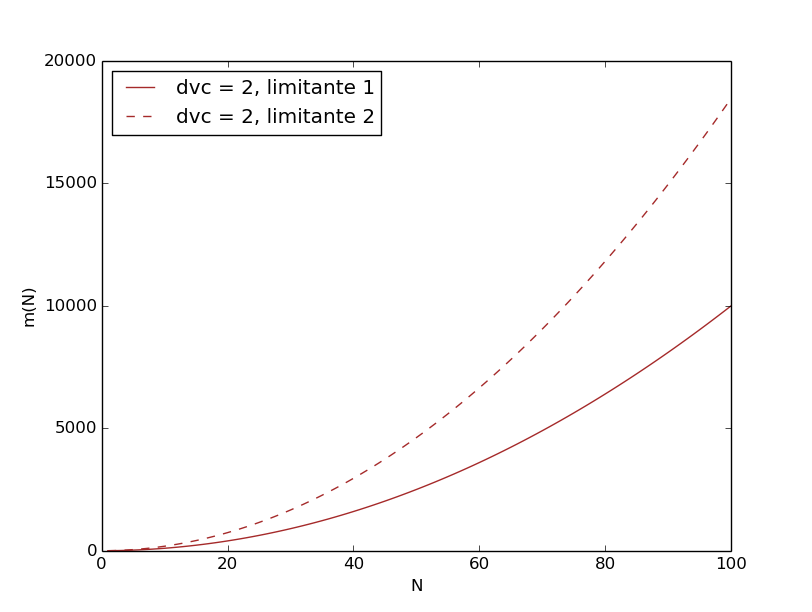
\includegraphics[width=\textwidth]{images/2-7-dvc2.png}
\caption{$\dvc = 2$}
\end{minipage}
\begin{minipage}{0.45\textwidth}
\centering
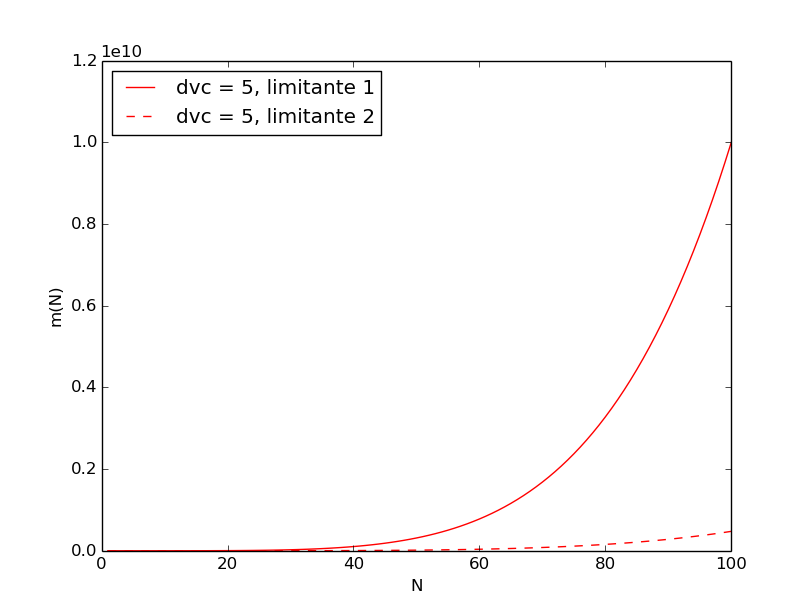
\includegraphics[width=\textwidth]{images/2-7-dvc5.png}
\caption{$\dvc = 5$}
\end{minipage}
\end{figure}

\begin{center}
Limitante 1: $m_{\hipotset}(N) \le N^{\dvc} + 1$

Limitante 2: $m_{\hipotset}(N) \le \left( \frac{eN}{\dvc} \right)^{\dvc}$
\end{center}


O limitante 1 é melhor que o limitante 2 quando $\dvc \le e$, por isso o resultado observado no primeiro gráfico, quando $\dvc = 2$. Para valores maiores de $\dvc$, basta observar que $\left( \frac{eN}{\dvc} \right) \le N$ quando $\dvc \ge e$, e então o segundo limitante é melhor.
